% Compile from the repository root with:
%   pdflatex -interaction=nonstopmode -halt-on-error -output-directory=report report/TRYOPS_MLOPS_FINAL_REPORT_VI.tex
\documentclass[12pt,a4paper,oneside]{report}

\usepackage[a4paper,top=2.5cm,bottom=2.5cm,left=2.8cm,right=2.2cm]{geometry}
\usepackage[utf8]{inputenc}
\usepackage[T5]{fontenc}
\usepackage{lmodern}
\usepackage{graphicx}
\usepackage{xcolor}
\usepackage{array}
\usepackage{booktabs}
\usepackage{longtable}
\usepackage{tabularx}
\usepackage{enumitem}
\usepackage{fancyhdr}
\usepackage{titlesec}
\usepackage{hyperref}
\usepackage{listings}
\usepackage{tikz}
\usepackage{float}
\usepackage{caption}
\usetikzlibrary{arrows.meta,positioning,fit,shapes.geometric,calc}

\graphicspath{
  {./}
  {report/assets/}
  {assets/}
}

\definecolor{TryOpsNavy}{HTML}{111827}
\definecolor{TryOpsInk}{HTML}{1F2937}
\definecolor{TryOpsBlue}{HTML}{2563EB}
\definecolor{TryOpsTeal}{HTML}{0F766E}
\definecolor{TryOpsGold}{HTML}{B45309}
\definecolor{TryOpsRed}{HTML}{B91C1C}
\definecolor{TryOpsSlate}{HTML}{475569}
\definecolor{TryOpsMist}{HTML}{F8FAFC}
\definecolor{TryOpsLine}{HTML}{CBD5E1}
\definecolor{CodeBg}{HTML}{F8FAFC}

\hypersetup{
  unicode=true,
  colorlinks=true,
  linkcolor=TryOpsBlue,
  urlcolor=TryOpsTeal,
  citecolor=TryOpsBlue,
  pdftitle={TryOps: Nen tang MLOps cho Virtual Try-On va LLM Serving},
  pdfauthor={Nguyen Tran Nhat Trung, Hoang Minh Thai, Pham Hai Dang}
}

\pagestyle{fancy}
\fancyhf{}
\lhead{\small TryOps MLOps}
\rhead{\small Group1.CS317}
\cfoot{\thepage}
\setlength{\headheight}{14pt}
\renewcommand{\headrulewidth}{0.4pt}

\titleformat{\chapter}
  {\normalfont\huge\bfseries\color{TryOpsNavy}}
  {\thechapter.}{0.8em}{}
\titleformat{\section}
  {\normalfont\Large\bfseries\color{TryOpsNavy}}
  {\thesection}{0.7em}{}
\titleformat{\subsection}
  {\normalfont\large\bfseries\color{TryOpsNavy}}
  {\thesubsection}{0.6em}{}

\setlist[itemize]{leftmargin=1.1cm,itemsep=0.25em,topsep=0.25em}
\setlist[enumerate]{leftmargin=1.1cm,itemsep=0.25em,topsep=0.25em}
\renewcommand{\arraystretch}{1.22}
\setlength{\parindent}{0pt}
\setlength{\parskip}{0.55em}

\renewcommand{\contentsname}{Mục lục}
\renewcommand{\listfigurename}{Danh sách hình}
\renewcommand{\figurename}{Hình}
\renewcommand{\tablename}{Bảng}
\renewcommand{\bibname}{Tài liệu tham khảo}

\newcommand{\code}[1]{\texttt{\detokenize{#1}}}
\newcommand{\reporttitle}{TryOps: Nền tảng MLOps cho Virtual Try-On và LLM Serving}
\newcommand{\reportsubtitle}{Governance, Model Serving, Observability và Vận hành hệ thống học máy}
\newcommand{\metric}[2][TryOpsBlue]{\textbf{\color{#1}#2}}

\lstdefinestyle{tryopscode}{
  basicstyle=\small\ttfamily,
  backgroundcolor=\color{CodeBg},
  frame=single,
  rulecolor=\color{TryOpsLine},
  breaklines=true,
  columns=fullflexible,
  keepspaces=true,
  showstringspaces=false,
  tabsize=2
}
\lstset{style=tryopscode}

\newcommand{\metriccard}[4][TryOpsBlue]{%
  \fcolorbox{#1!35}{#1!7}{%
    \begin{minipage}[t]{#2}
      \centering
      {\scriptsize\bfseries\color{TryOpsSlate}#3\par}
      \vspace{0.10em}
      {\Large\bfseries\color{#1}#4\par}
    \end{minipage}%
  }%
}

\newcommand{\techlogo}[2]{%
  \begin{minipage}[t]{1.50cm}
    \centering
    \includegraphics[height=0.50cm,width=1.32cm,keepaspectratio]{#1}\\[-0.03cm]
    {\tiny #2}
  \end{minipage}\hspace{0.05cm}%
}

\newcommand{\screenshotfig}[2]{%
  \begin{figure}[H]
    \centering
    \includegraphics[width=\linewidth]{#1}
    \caption[#2]{#2.}
  \end{figure}
}

\begin{document}

% ---------------------------------------------------------------------------
% Cover
% ---------------------------------------------------------------------------
\begin{titlepage}
  \thispagestyle{empty}
  \centering
  \begin{tikzpicture}[remember picture,overlay]
    \draw[line width=1.7pt,color=TryOpsBlue]
      ([xshift=1.35cm,yshift=-1.35cm]current page.north west)
      rectangle
      ([xshift=-1.35cm,yshift=1.35cm]current page.south east);
    \draw[line width=0.65pt,color=TryOpsBlue]
      ([xshift=1.50cm,yshift=-1.50cm]current page.north west)
      rectangle
      ([xshift=-1.50cm,yshift=1.50cm]current page.south east);
    \draw[line width=0.55pt,color=TryOpsLine]
      ([xshift=1.78cm,yshift=-1.78cm]current page.north west)
      -- ++(1.45cm,0) arc[start angle=90,end angle=0,radius=0.45cm] -- ++(0,-1.45cm);
    \draw[line width=0.55pt,color=TryOpsLine]
      ([xshift=-1.78cm,yshift=1.78cm]current page.south east)
      -- ++(-1.45cm,0) arc[start angle=-90,end angle=-180,radius=0.45cm] -- ++(0,1.45cm);
  \end{tikzpicture}

  \vspace*{-0.25cm}
  {\bfseries\Large ĐẠI HỌC QUỐC GIA TP. HỒ CHÍ MINH\par}
  \vspace{0.20cm}
  {\bfseries\Large TRƯỜNG ĐẠI HỌC CÔNG NGHỆ THÔNG TIN\par}
  \vspace{0.20cm}
  {\bfseries\large KHOA KHOA HỌC MÁY TÍNH\par}

  \vspace{0.70cm}
  
\includegraphics[height=3.1cm,trim=0 305 0 0,clip]{uit-emblem.png}\par

  \vspace{0.72cm}
  {\bfseries\large MÔN HỌC\par}
  \vspace{0.18cm}
  {\large CS317.Q22 -- PHÁT TRIỂN VÀ VẬN HÀNH HỆ THỐNG HỌC MÁY\par}

  \vspace{0.72cm}
  {\bfseries\large BÁO CÁO ĐỒ ÁN CUỐI KỲ\par}
  \vspace{0.28cm}
  \begin{minipage}{0.84\textwidth}
    \centering
    {\bfseries\Large\color{TryOpsNavy}\reporttitle\par}
  \end{minipage}
  \vspace{0.26cm}

  {\normalsize\textbf{Repository:} \href{https://github.com/trungdangtapcode/TryOps-TryON-MLOps}{github.com/trungdangtapcode/TryOps-TryON-MLOps}\par}

  \vspace{0.58cm}
  \begin{tabular}{>{\bfseries\raggedright\arraybackslash}p{4.9cm}p{6.5cm}}
    Giảng viên hướng dẫn: & MSc. Đỗ Văn Tiến \\
    Trợ giảng: & Lê Trần Trọng Khiêm \\
  \end{tabular}

  \vspace{0.58cm}
  \begin{tabular}{>{\bfseries}p{2.2cm}p{6.4cm}p{2.9cm}}
    Sinh viên: & Nguyễn Trần Nhật Trung & 23521684 \\
               & Hoàng Minh Thái & 23521414 \\
               & Phạm Hải Đăng & 23520233 \\
  \end{tabular}

  \vfill
  {\large TP. Hồ Chí Minh, tháng 07 năm 2026\par}
\end{titlepage}

\pagenumbering{roman}

\chapter*{Tóm tắt}
\addcontentsline{toc}{chapter}{Tóm tắt}

TryOps là một nền tảng MLOps được xây dựng quanh hai workload có yêu cầu vận hành cao: Virtual Try-On (VTON) và Large Language Model (LLM) serving. Trọng tâm của đồ án không chỉ là tạo ra một kết quả inference, mà là xây dựng hệ thống xung quanh vòng đời của model: dữ liệu, artifact, endpoint cấu hình, account, quota, asynchronous job, policy gate, model registry, observability, rollback posture và các record cần thiết cho việc kiểm tra vận hành.

Hệ thống gồm bốn lớp chính. Lớp product là React/Vite console, hỗ trợ đăng nhập, workspace, VTON Studio, LLM Playground, model registry, governance, dashboard và history. Lớp edge là Rust Axum gateway, chịu trách nhiệm authentication, proxying, request limit, quota admission, guardrail dispatch, static serving và Prometheus metrics. Lớp workflow là FastAPI backend, quản lý product API, VTON job orchestration, artifact metadata, evaluation, account state và governance view. Lớp inference/control-plane gồm host-side FASHN VTON router và worker, OpenAI-compatible LLM endpoint, Go service, cùng C++ native tools cho policy, metrics, SLO check, supply-chain record, cache, energy và evaluation.

Đóng góp chính của TryOps là đặt workload AI vào một operational boundary rõ ràng. VTON cần GPU-aware job control, image artifact lineage và kiểm tra chất lượng ảnh. LLM serving cần token accounting, endpoint health, guardrail và latency/cost measurement. TryOps dùng chung một nền tảng gateway, API, storage, observability và governance cho cả hai nhóm workload.

Phiên bản hiện tại hỗ trợ developer-local stack với Postgres, Valkey, MinIO, MLflow, Keycloak, FastAPI, Rust gateway, Go guardrail, Prometheus, Grafana, Loki, Tempo, OpenTelemetry Collector và FASHN VTON router chạy phía host. Báo cáo này trình bày kiến trúc, yêu cầu, thiết kế model serving, governance, observability, port topology, benchmark VTON/LLM và các giới hạn còn lại.

\textbf{Từ khóa:} MLOps, Virtual Try-On, FASHN VTON, LLM Serving, vLLM, OpenAI-compatible API, Rust Gateway, FastAPI, Go, C++, Prometheus, Grafana, Loki, Tempo, MLflow, MinIO, Keycloak, governance, policy gate.

\tableofcontents
\listoffigures
\clearpage
\pagenumbering{arabic}

% ---------------------------------------------------------------------------
\chapter{Giới thiệu}
% ---------------------------------------------------------------------------

\section{Động lực}

Nhiều ứng dụng học máy có thể tạo ra một ảnh kết quả hoặc một đoạn văn trả lời có vẻ thuyết phục. Tuy nhiên, một hệ thống ML được vận hành nghiêm túc phải trả lời được các câu hỏi ngoài phạm vi notebook:

\begin{itemize}
  \item Dữ liệu, model weights, code version, configuration và phần cứng nào đã tạo ra output?
  \item Candidate model có bị chặn trước khi tới người dùng nếu không đạt policy hay không?
  \item Khi endpoint đã cấu hình không sẵn sàng, hệ thống có trả operational error rõ ràng không?
  \item Mỗi workspace có được kiểm soát bằng quota, rate limit và concurrency limit không?
  \item Operator có debug được lỗi bằng metrics, logs, traces, job ID và request ID không?
  \item Release có thể rollback và giải thích lại cho reviewer không?
\end{itemize}

TryOps được thiết kế để trả lời các câu hỏi trên. Hai workload được chọn có tính chất khác nhau: VTON là workload thị giác, nặng GPU, nhạy về quyền riêng tư ảnh người dùng và khó đánh giá vì lỗi thường mang tính cảm nhận; LLM serving nhạy với latency, throughput, token cost, guardrail và prompt injection. Nếu một nền tảng có thể vận hành cả hai workload này trong cùng một governance spine, nền tảng đó thể hiện rõ tư duy MLOps hơn một ứng dụng đơn lẻ.

\section{Mục tiêu đồ án}

Mục tiêu của đồ án là xây dựng một nền tảng MLOps có thể vận hành workload AI với traceability, observability, quota và governance.

Các mục tiêu cụ thể:

\begin{enumerate}
  \item Xây dựng TryOps Console cho end user, operator và reviewer.
  \item Dùng Rust gateway làm edge boundary.
  \item Dùng FastAPI làm product workflow backend và model adapter layer.
  \item Chạy VTON qua FASHN VTON serving path.
  \item Hỗ trợ LLM inference qua OpenAI-compatible endpoint, bao gồm self-hosted vLLM hoặc managed API.
  \item Tích hợp Keycloak cho OIDC login và workspace identity.
  \item Tích hợp Postgres, Valkey, MinIO và MLflow cho product data, counter, object storage và experiment tracking.
  \item Tích hợp Prometheus, Grafana, Loki, Tempo và OpenTelemetry cho observability.
  \item Cài đặt governance thông qua policy gate, supply-chain record, model card, data card và promotion record.
  \item Tách bạch utility cho testing/evaluation khỏi product inference path.
\end{enumerate}

\section{Hướng phát triển}

\begin{longtable}{p{3.0cm}p{5.55cm}p{5.55cm}}
\toprule
\textbf{Nhóm} & \textbf{Hiện tại} & \textbf{Tương lai} \\
\midrule
Product & TryOps Console, LLM Playground, VTON Studio, Account, Registry, Governance, Dashboard, History & Bổ sung accessibility, export workflow và nhiều operator action hơn \\
VTON & FASHN VTON router, GPU worker, image upload, async job, artifact output, metrics & Human preference study và model zoo rộng hơn \\
LLM & OpenAI-compatible endpoint, OpenAI/vLLM configuration, guardrail, quota & Live vLLM benchmark phụ thuộc workspace và GPU khả dụng \\
MLOps & MLflow, MinIO, promotion record, model/data card, policy gate & KServe/Kubeflow deployment profile \\
Observability & Prometheus, Grafana, Loki, Tempo, OTel bridge, structured logs & GPU/process exporter đầy đủ cho nhiều biến thể shared-datacenter \\
Security & Keycloak, gateway auth, quota, guardrail, supply-chain record & External Secrets/Vault cho production cluster \\
Networking & Developer-local port map và shared-datacenter plan & Ingress/hardening profile cuối cùng cho multi-tenant data center \\
\bottomrule
\end{longtable}

\section{Đặc điểm kỹ thuật}

\begin{itemize}
  \item Một local deployment path có thể triển khai cho full product stack trên GCP hoặc AWS.
  \item Native-first boundary: Rust ở edge, Go cho service/controller/load tool, C++ cho native tools, Python cho ML workflow.
  \item VTON serving abstraction: API gọi một endpoint ổn định, router ẩn worker count, GPU mapping, socket và per-worker metrics.
  \item LLM adapter dùng OpenAI-compatible API và endpoint-error handling rõ ràng.
  \item Observability stack gồm Grafana dashboard, Loki logs, Tempo traces, Prometheus metrics và structured job/request logs.
  \item Governance pipeline gồm policy gate, supply-chain record, dependency lock, model scan, provenance và promotion lifecycle record.
\end{itemize}

\section{Technology Stack}

\begin{figure}[H]
  \centering
  \small
  \setlength{\tabcolsep}{5pt}
  \renewcommand{\arraystretch}{1.5}
  \begin{tabularx}{\linewidth}{>{\raggedright\arraybackslash\bfseries\color{TryOpsNavy}}p{2.85cm}X}
    Product UI &
      \techlogo{logos/react.png}{React}
      \techlogo{logos/typescript.png}{TypeScript}
      \techlogo{logos/vite.png}{Vite}
      \techlogo{logos/lucide.png}{Lucide}
      \techlogo{logos/tailwind.png}{Tailwind} \\
    API and Native Runtime &
      \techlogo{logos/python.png}{Python}
      \techlogo{logos/fastapi.png}{FastAPI}
      \techlogo{logos/rust.png}{Rust}
      \techlogo{logos/go.png}{Go}
      \techlogo{logos/cplusplus.png}{C++}
      \techlogo{logos/docker.png}{Docker} \\
    Data, Identity, and Governance &
      \techlogo{logos/postgresql.png}{Postgres}
      \techlogo{logos/valkey.png}{Valkey}
      \techlogo{logos/minio.png}{MinIO}
      \techlogo{logos/mlflow.png}{MLflow}
      \techlogo{logos/dvc.png}{DVC}
      \techlogo{logos/keycloak.png}{Keycloak} \\
    Model Serving and AI Libraries &
      \techlogo{logos/pytorch.png}{PyTorch}
      \techlogo{logos/huggingface.png}{HF Hub}
      \techlogo{logos/fashn.png}{FASHN VTON}
      \techlogo{logos/openai.png}{OpenAI API}
      \techlogo{logos/vllm.png}{vLLM} \\
    Observability and Operations &
      \techlogo{logos/prometheus.png}{Prometheus}
      \techlogo{logos/grafana.png}{Grafana}
      \techlogo{logos/loki.png}{Loki}
      \techlogo{logos/tempo.png}{Tempo}
      \techlogo{logos/opentelemetry.png}{OTel}
      \techlogo{logos/alertmanager.png}{Alertmanager} \\
  \end{tabularx}
  \caption{Technology stack của TryOps theo từng lớp sản phẩm.}
\end{figure}

% ---------------------------------------------------------------------------
\chapter{Cơ sở kỹ thuật và yêu cầu MLOps}
% ---------------------------------------------------------------------------

\section{MLOps trong hệ thống AI}

MLOps là tập hợp quy trình và công cụ để đưa model từ giai đoạn thử nghiệm sang vận hành có kiểm soát. Trong đồ án này, các yêu cầu MLOps quan trọng gồm:

\begin{itemize}
  \item Versioning cho data, code, configuration và model artifact.
  \item Experiment tracking và artifact storage.
  \item Evaluation trước khi promotion.
  \item Model registry với lifecycle state: candidate, challenger, champion, rejected, archived.
  \item CI/CD và policy gate.
  \item Observability cho metrics, logs, traces, drift, quality và cost.
  \item Security, quota, guardrail và rollback.
\end{itemize}

TryOps hiện thực các yêu cầu trên bằng MLflow, MinIO, Postgres, Valkey, generated reports, runtime artifacts, native policy/evaluation tools và Grafana/Loki/Tempo dashboards.

\section{Virtual Try-On}

Virtual Try-On nhận ảnh người và ảnh trang phục, sau đó sinh ảnh người mặc trang phục đó. Đây là workload khó vận hành vì:

\begin{itemize}
  \item Output là ảnh, lỗi có thể là méo hình, identity drift, mất texture, sai pose, hỏng chi tiết cơ thể hoặc artifact tại vùng biên trang phục.
  \item GPU memory và latency có thể lớn.
  \item Ảnh người dùng có tính riêng tư cao.
  \item Hệ thống phải lưu input, output, report metadata, metrics và lineage.
  \item Hệ thống phải biết output được tạo từ product path hay từ evaluation utility.
\end{itemize}

TryOps sử dụng FASHN VTON v1.5 cho VTON serving. Theo tài liệu nghiên cứu của FASHN, VTON v1.5 là maskless pixel-space virtual try-on model, hướng tới việc giữ chi tiết trang phục mà không cần segmentation mask thủ công \cite{fashn-vton}.

\section{LLM Serving}

LLM serving cần theo dõi latency, throughput, token count, token cost, quota, cache effect, guardrail outcome và endpoint failure. TryOps chuẩn hóa LLM serving thông qua OpenAI-compatible API. Endpoint có thể là self-hosted vLLM hoặc managed provider, nhưng product contract vẫn giống nhau: request đi qua gateway, backend ghi lại metadata cần thiết, provider secret được đưa vào runtime configuration, và lỗi endpoint được đưa vào observability stack.

% ---------------------------------------------------------------------------
\chapter{Phân tích yêu cầu}
% ---------------------------------------------------------------------------

\section{Actor}

\begin{longtable}{p{4.1cm}p{10.6cm}}
\toprule
\textbf{Actor} & \textbf{Nhu cầu} \\
\midrule
End user & Login, upload ảnh, chạy try-on, xem trạng thái job, mở kết quả \\
ML engineer & Chạy benchmark, so sánh candidate, xem evaluation report \\
Platform engineer & Vận hành stack, xem logs/metrics/traces, cấu hình endpoint và port \\
Risk reviewer & Kiểm tra model card, data card, policy gate, supply-chain record và lineage \\
Admin/operator & Theo dõi quota, account, registry state, incident và rollback record \\
Evaluator/instructor & Kiểm tra behavior qua code, dashboard, artifact, report và kết quả benchmark \\
\bottomrule
\end{longtable}

\section{Yêu cầu chức năng}

Các yêu cầu chức năng được chia theo module để làm rõ trách nhiệm của từng phần trong hệ thống. Cách đánh mã \code{FR-*} giúp liên kết yêu cầu với thiết kế, kiểm thử, dashboard và phần đánh giá ở các chương sau.

\subsection{Module TryOps Console và Workspace}

\begingroup
\small
\begin{longtable}{p{2.05cm}p{4.05cm}p{8.05cm}}
\caption{Yêu cầu chức năng -- Module TryOps Console và Workspace.}\\
\toprule
\textbf{ID} & \textbf{Yêu cầu} & \textbf{Mô tả} \\
\midrule
\endfirsthead
\toprule
\textbf{ID} & \textbf{Yêu cầu} & \textbf{Mô tả} \\
\midrule
\endhead
FR-UI-01 & Đăng nhập và session & User đăng nhập qua Keycloak/OIDC; frontend nhận trạng thái session và gửi request qua Rust gateway. \\
FR-UI-02 & Workspace context & UI hiển thị workspace hiện tại, account name, plan/quota và trạng thái sử dụng tài nguyên. \\
FR-UI-03 & Điều hướng sản phẩm & User chuyển được giữa Studio, Account, Registry, Governance, Dashboard và History. \\
FR-UI-04 & Job visibility & UI hiển thị active, queued, completed và failed job; user có thể xem lại output và trạng thái job sau khi thao tác. \\
FR-UI-05 & Feedback và history & User có thể xem request history, job history và gửi feedback cho kết quả model. \\
\bottomrule
\end{longtable}
\endgroup

\subsection{Module VTON Workflow}

\begingroup
\small
\begin{longtable}{p{2.05cm}p{4.05cm}p{8.05cm}}
\caption{Yêu cầu chức năng -- Module VTON Workflow.}\\
\toprule
\textbf{ID} & \textbf{Yêu cầu} & \textbf{Mô tả} \\
\midrule
\endfirsthead
\toprule
\textbf{ID} & \textbf{Yêu cầu} & \textbf{Mô tả} \\
\midrule
\endhead
FR-VTON-01 & Upload ảnh đầu vào & User upload person image và garment image; API kiểm tra định dạng, lưu artifact và trả metadata cho UI. \\
FR-VTON-02 & Cấu hình try-on & User chọn garment category, source type và quality mode trước khi submit job. \\
FR-VTON-03 & Submit async job & Backend tạo VTON job bất đồng bộ, kiểm tra quota/concurrency và lưu job snapshot. \\
FR-VTON-04 & Theo dõi job status & UI poll trạng thái \code{accepted}, \code{queued}, \code{running}, \code{completed} hoặc \code{failed}. \\
FR-VTON-05 & Gọi model serving & VTON adapter gửi request tới FASHN router endpoint đã cấu hình; router dispatch tới GPU worker. \\
FR-VTON-06 & Lưu output artifact & Khi job hoàn tất, hệ thống lưu output image, report metadata, latency và lineage. \\
FR-VTON-07 & Hiển thị kết quả & UI hiển thị generated image, job duration, trạng thái và link artifact cho user. \\
\bottomrule
\end{longtable}
\endgroup

\subsection{Module LLM Serving}

\begingroup
\small
\begin{longtable}{p{2.05cm}p{4.05cm}p{8.05cm}}
\caption{Yêu cầu chức năng -- Module LLM Serving.}\\
\toprule
\textbf{ID} & \textbf{Yêu cầu} & \textbf{Mô tả} \\
\midrule
\endfirsthead
\toprule
\textbf{ID} & \textbf{Yêu cầu} & \textbf{Mô tả} \\
\midrule
\endhead
FR-LLM-01 & Gửi prompt & User gửi prompt từ LLM Playground; request đi qua gateway, guardrail và FastAPI backend. \\
FR-LLM-02 & Gọi OpenAI-compatible endpoint & Backend gọi configured OpenAI-compatible endpoint, bao gồm managed provider hoặc self-hosted vLLM. \\
FR-LLM-03 & Ghi metadata & Hệ thống ghi model name, provider, token count, latency, tokens/s và cost estimate khi có cấu hình. \\
FR-LLM-04 & Guardrail outcome & Guardrail có thể allow, redact, review hoặc block request/response theo policy. \\
FR-LLM-05 & Lưu request history & Prompt metadata, response metadata và trạng thái được lưu để user/operator xem lại. \\
\bottomrule
\end{longtable}
\endgroup

\subsection{Module Governance và Registry}

\begingroup
\small
\begin{longtable}{p{2.05cm}p{4.05cm}p{8.05cm}}
\caption{Yêu cầu chức năng -- Module Governance và Registry.}\\
\toprule
\textbf{ID} & \textbf{Yêu cầu} & \textbf{Mô tả} \\
\midrule
\endfirsthead
\toprule
\textbf{ID} & \textbf{Yêu cầu} & \textbf{Mô tả} \\
\midrule
\endhead
FR-GOV-01 & Model registry view & Operator xem model lifecycle state như candidate, challenger, champion, rejected và archived. \\
FR-GOV-02 & Model card và data card & Reviewer xem metadata về model source, dataset, owner, intended use và risk note. \\
FR-GOV-03 & Promotion gate & Hệ thống lưu policy verdict, evaluation report, SBOM, scan result, provenance và approval record. \\
FR-GOV-04 & Rollback record & Operator xem candidate/champion history để phục vụ rollback và audit. \\
FR-GOV-05 & Supply-chain record & Hệ thống lưu dependency lock, model-source pin và artifact provenance cho release. \\
\bottomrule
\end{longtable}
\endgroup

\subsection{Module Observability và Operations}

\begingroup
\small
\begin{longtable}{p{2.05cm}p{4.05cm}p{8.05cm}}
\caption{Yêu cầu chức năng -- Module Observability và Operations.}\\
\toprule
\textbf{ID} & \textbf{Yêu cầu} & \textbf{Mô tả} \\
\midrule
\endfirsthead
\toprule
\textbf{ID} & \textbf{Yêu cầu} & \textbf{Mô tả} \\
\midrule
\endhead
FR-OPS-01 & Service dashboard & Grafana hiển thị request rate, error rate, latency, memory, queue depth và gateway errors. \\
FR-OPS-02 & Log drilldown & Operator tìm log theo job ID, request ID, account ID, worker ID và GPU ID. \\
FR-OPS-03 & Trace và metrics & OpenTelemetry, Tempo và Prometheus ghi trace/metric cho API, gateway, router và worker. \\
FR-OPS-04 & Alerting & Prometheus/Alertmanager hỗ trợ rule cho service health, error rate và latency. \\
FR-OPS-05 & Startup và port map & Hệ thống có developer-local port table, health check và startup output để operator biết entry point. \\
\bottomrule
\end{longtable}
\endgroup

\section{Yêu cầu phi chức năng}

\begingroup
\small
\begin{longtable}{p{2.05cm}p{4.25cm}p{7.85cm}}
\caption{Yêu cầu phi chức năng của TryOps.}\\
\toprule
\textbf{ID} & \textbf{Yêu cầu} & \textbf{Tiêu chí} \\
\midrule
\endfirsthead
\toprule
\textbf{ID} & \textbf{Yêu cầu} & \textbf{Tiêu chí} \\
\midrule
\endhead
NFR-01 & Security & User request đi qua Keycloak/OIDC và Rust gateway; development shortcut không được dùng cho deployment nghiêm túc. \\
NFR-02 & Privacy & Logs không lưu raw prompt, raw uploaded image hoặc provider secret; log dùng job ID, request ID và artifact ID. \\
NFR-03 & Observability & Mỗi workflow quan trọng có metrics, logs và traces; Grafana hỗ trợ drilldown cho job lỗi. \\
NFR-04 & Endpoint readiness & VTON/LLM adapter phải báo lỗi rõ khi configured endpoint không sẵn sàng để operator xử lý hạ tầng. \\
NFR-05 & Scalability & FASHN router hỗ trợ nhiều GPU worker, per-worker metrics và routing theo in-flight state. \\
NFR-06 & Performance & Benchmark ghi average latency, P95 latency, throughput, GPU utilization và VRAM để so sánh candidate. \\
NFR-07 & Reproducibility & Model/data/config/code/artifact có record; evaluation và promotion report có thể truy vết lại. \\
NFR-08 & Operability & Stack có health check, startup output, port map, dashboard và log drilldown để debug trong vận hành. \\
NFR-09 & Shared-host networking & Public surface nên thu hẹp về gateway, Keycloak và admin-restricted Grafana; internal services nằm trong private network. \\
NFR-10 & Governance & Promotion cần model card, data card, policy verdict, scan result, provenance và owner approval. \\
\bottomrule
\end{longtable}
\endgroup

\section{Luồng xử lý chính}

\subsection{Luồng Virtual Try-On}

\begin{enumerate}
  \item User đăng nhập và mở TryOps Studio trong workspace.
  \item User upload person image và garment image.
  \item UI gửi metadata cấu hình gồm garment category, source type và quality mode.
  \item Backend kiểm tra authentication, quota và workspace concurrency.
  \item Backend tạo VTON job bất đồng bộ và lưu job snapshot.
  \item Runner gọi FASHN router endpoint để thực hiện model serving.
  \item Router dispatch request tới GPU worker phù hợp.
  \item Worker sinh output image; backend lưu output artifact, report metadata và lineage.
  \item UI poll job status và hiển thị kết quả khi job completed.
\end{enumerate}

\subsection{Luồng LLM Request}

\begin{enumerate}
  \item User nhập prompt từ LLM Playground.
  \item Gateway kiểm tra identity, rate limit và quota admission.
  \item Guardrail đánh giá request theo policy.
  \item Backend gọi OpenAI-compatible endpoint đã cấu hình.
  \item Hệ thống ghi latency, token count, model metadata và guardrail outcome.
  \item UI hiển thị response hoặc operational error tương ứng.
\end{enumerate}

\subsection{Luồng Model Promotion}

\begin{enumerate}
  \item ML engineer tạo candidate từ benchmark/evaluation run.
  \item Hệ thống lưu artifact, model card, data card và evaluation report.
  \item Policy gate kiểm tra quality, security, provenance và approval.
  \item Candidate đạt yêu cầu được chuyển sang challenger hoặc champion.
  \item Candidate không đạt yêu cầu được ghi rejection record để reviewer kiểm tra.
\end{enumerate}

\section{Ranh giới Product và Diagnostics}

\begin{longtable}{p{3.1cm}p{5.55cm}p{5.55cm}}
\toprule
\textbf{Component} & \textbf{Product path} & \textbf{Diagnostics/evaluation utility} \\
\midrule
VTON & FASHN router qua configured VTON serving endpoint & Overlay/image utility chỉ dùng khi bật rõ cho test \\
LLM & OpenAI-compatible model endpoint & Harness cho adapter check \\
Semantic cache & Feature có cấu hình và có quan sát & Tắt trong cấu hình ưu tiên an toàn \\
API keys & OIDC/JWT và provider secret & Static development key tắt trong cấu hình mặc định \\
Worker ports & Ẩn sau router & Direct worker port chỉ dùng để debug \\
\bottomrule
\end{longtable}

Ranh giới này giúp báo cáo đúng năng lực của hệ thống: phần product path phục vụ user, còn diagnostics/evaluation utility phục vụ kiểm thử, đo đạc và phân tích.

% ---------------------------------------------------------------------------
\chapter{Kiến trúc hệ thống}
% ---------------------------------------------------------------------------

\section{Tổng quan kiến trúc}

\begin{figure}[H]
\centering
\scriptsize
\resizebox{\linewidth}{!}{%
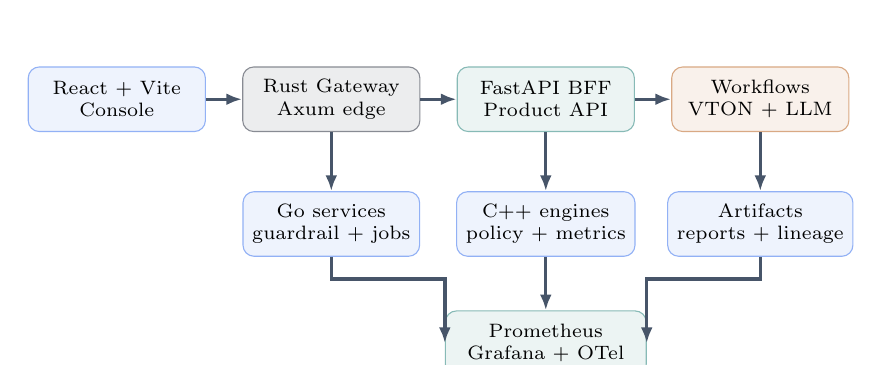
\begin{tikzpicture}[
  node distance=0.38cm and 0.46cm,
  every node/.style={font=\scriptsize},
  boundary/.style={draw=#1!50, fill=#1!8, rounded corners=4pt, minimum width=2.25cm, minimum height=0.82cm, align=center},
  arrow/.style={-{Latex[length=2mm]}, very thick, color=TryOpsSlate}
]
\node[boundary=TryOpsBlue] (web) {React + Vite\\Console};
\node[boundary=TryOpsNavy, right=of web] (gateway) {Rust Gateway\\Axum edge};
\node[boundary=TryOpsTeal, right=of gateway] (api) {FastAPI BFF\\Product API};
\node[boundary=TryOpsGold, right=of api] (workflows) {Workflows\\VTON + LLM};

\node[boundary=TryOpsBlue, minimum width=2.05cm, below=0.75cm of gateway] (go) {Go services\\guardrail + jobs};
\node[boundary=TryOpsBlue, minimum width=2.05cm, below=0.75cm of api] (cpp) {C++ engines\\policy + metrics};
\node[boundary=TryOpsBlue, minimum width=2.05cm, below=0.75cm of workflows] (store) {Artifacts\\reports + lineage};
\node[boundary=TryOpsTeal, minimum width=2.55cm, below=0.68cm of cpp] (obs) {Prometheus\\Grafana + OTel};

\draw[arrow] (web) -- (gateway);
\draw[arrow] (gateway) -- (api);
\draw[arrow] (api) -- (workflows);
\draw[arrow] (gateway) -- (go);
\draw[arrow] (api) -- (cpp);
\draw[arrow] (workflows) -- (store);
\draw[arrow] (go.south) -- ++(0,-0.28) -| (obs.west);
\draw[arrow] (cpp.south) -- (obs.north);
\draw[arrow] (store.south) -- ++(0,-0.28) -| (obs.east);
\end{tikzpicture}%
}

\vspace{0.45em}
\begin{minipage}[t]{0.48\linewidth}
\fcolorbox{TryOpsBlue!22}{TryOpsBlue!5}{%
  \begin{minipage}{0.94\linewidth}
  \textbf{Compiled product boundary}\par
  Rust xử lý \code{/api/*}; Go đảm nhận sidecar và controller-style service; C++ hỗ trợ native tools.
  \end{minipage}}
\end{minipage}\hfill
\begin{minipage}[t]{0.48\linewidth}
\fcolorbox{TryOpsTeal!22}{TryOpsTeal!5}{%
  \begin{minipage}{0.94\linewidth}
  \textbf{Python role}\par
  Python điều phối ML workflow và product API; các phần policy/metrics quan trọng được mirror hoặc chuyển sang native tools khi cần.
  \end{minipage}}
\end{minipage}
\caption{Product boundary architecture của TryOps.}
\end{figure}

\begin{figure}[H]
\centering
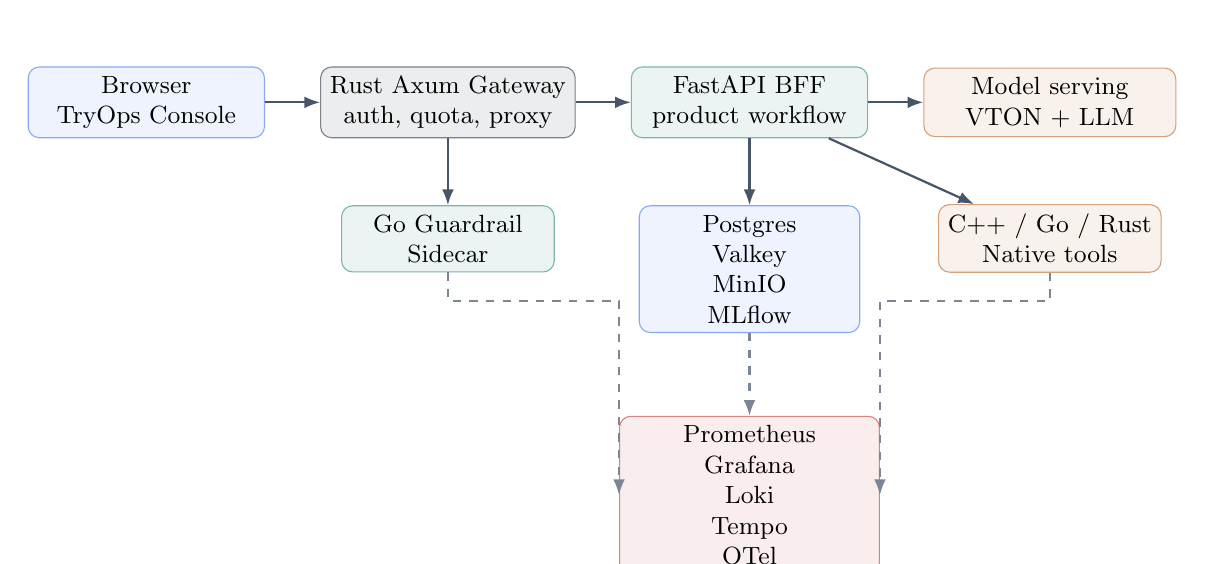
\begin{tikzpicture}[
  node distance=0.85cm and 0.7cm,
  box/.style={draw=#1!55, fill=#1!8, rounded corners=4pt, minimum height=0.84cm, align=center, font=\small},
  arrow/.style={-{Latex[length=2mm]}, thick, color=TryOpsSlate},
  telemetry/.style={-{Latex[length=2mm]}, thick, dashed, color=TryOpsSlate!72}
]
\node[box=TryOpsBlue, minimum width=3.0cm] (user) {Browser\\TryOps Console};
\node[box=TryOpsNavy, minimum width=3.2cm, right=of user] (gateway) {Rust Axum Gateway\\auth, quota, proxy};
\node[box=TryOpsTeal, minimum width=3.0cm, right=of gateway] (api) {FastAPI BFF\\product workflow};
\node[box=TryOpsGold, minimum width=3.2cm, right=of api] (models) {Model serving\\VTON + LLM};

\node[box=TryOpsTeal, minimum width=2.7cm, below=of gateway] (guardrail) {Go Guardrail\\Sidecar};
\node[box=TryOpsBlue, minimum width=2.8cm, below=of api] (data) {Postgres\\Valkey\\MinIO\\MLflow};
\node[box=TryOpsGold, minimum width=2.8cm, below=of models] (native) {C++ / Go / Rust\\Native tools};
\node[box=TryOpsRed, minimum width=3.3cm, below=1.05cm of data] (obs) {Prometheus\\Grafana\\Loki\\Tempo\\OTel};

\draw[arrow] (user) -- (gateway);
\draw[arrow] (gateway) -- (api);
\draw[arrow] (api) -- (models);
\draw[arrow] (gateway) -- (guardrail);
\draw[arrow] (api) -- (data);
\draw[arrow] (api) -- (native);
\draw[telemetry] (guardrail.south) -- ++(0,-0.36) -| (obs.west);
\draw[telemetry] (data.south) -- (obs.north);
\draw[telemetry] (native.south) -- ++(0,-0.36) -| (obs.east);
\end{tikzpicture}
\caption{Layered architecture của TryOps.}
\end{figure}

\section{Frontend Layer}

Frontend được tổ chức theo workflow sản phẩm, không chỉ là trang thử nghiệm đơn lẻ. Các chức năng chính:

\begin{itemize}
  \item VTON image upload, garment/source/quality selection và async job submission.
  \item Trình bày active, queued, completed và failed job.
  \item Gallery cho VTON output gần đây.
  \item LLM prompt workflow.
  \item Workspace quota và account state.
  \item Operator views cho dashboard, governance, registry, incident và rollback record.
  \item OIDC authorization-code flow với PKCE.
\end{itemize}

\screenshotfig{screenshots/main-page.png}{Giao diện TryOps Studio}
\screenshotfig{screenshots/workspace.png}{Workspace và quota view}
\screenshotfig{screenshots/example-run.png}{VTON job đang chạy trong UI}

\section{Gateway Layer}

Rust gateway là edge boundary của hệ thống:

\begin{itemize}
  \item Serve static UI assets.
  \item Proxy product API request tới workflow backend.
  \item Validate API key hoặc JWT/OIDC identity.
  \item Enforce rate limit và payload limit.
  \item Thực hiện quota admission trước khi chuyển tiếp workload tốn chi phí.
  \item Gọi Go guardrail sidecar trước LLM request.
  \item Forward request ID và trace context.
  \item Expose Prometheus metrics.
  \item Hỗ trợ TLS-oriented deployment profile.
\end{itemize}

Thiết kế này giúp Python không phải là security và quota boundary duy nhất.

\section{API và Workflow Layer}

FastAPI backend quản lý product workflow:

\begin{itemize}
  \item VTON image upload và async job management.
  \item LLM generation.
  \item Account/session API.
  \item Artifact read/write.
  \item Dashboard rollup.
  \item Request history và feedback.
  \item Promotion, evaluation, governance và lineage endpoints.
  \item Observability recording.
\end{itemize}

FastAPI không trực tiếp quản lý GPU scheduling. Nó gọi model serving thông qua URL ổn định.

\section{Data và Artifact Layer}

\begin{longtable}{p{4cm}p{10.5cm}}
\toprule
\textbf{Component} & \textbf{Vai trò} \\
\midrule
Postgres & Account, account member, request, job, quota ledger, artifact metadata \\
Valkey & Hot counter cho quota và rate limiting \\
MinIO & Object storage cho upload, output và MLflow artifact \\
MLflow & Experiment tracking và model registry record \\
DVC & Dataset và sample data versioning \\
Runtime artifact repository & Logs, reports, model weights, generated outputs \\
Generated reports repository & Promotion và evaluation reports \\
\bottomrule
\end{longtable}

\screenshotfig{screenshots/minIO.png}{MinIO artifact store}
\screenshotfig{screenshots/mlflow.png}{MLflow benchmark tracking}

\section{Observability Layer}

Telemetry source gồm:

\begin{itemize}
  \item FastAPI service metrics.
  \item Gateway service metrics.
  \item FASHN router và worker metrics.
  \item Go guardrail metrics.
  \item Structured API, router và worker logs.
  \item Trace span cho API và background job execution.
  \item OTel Collector và bridge components để export logs/traces tới Loki và Tempo.
\end{itemize}

\screenshotfig{screenshots/grafana.png}{Grafana observability dashboard}
\screenshotfig{screenshots/log-drilldown.png}{Log drilldown dashboard để debug job và request}

% ---------------------------------------------------------------------------
\chapter{Thiết kế Model Serving}
% ---------------------------------------------------------------------------

\section{VTON Serving}

VTON serving được tổ chức theo một serving path nhiều lớp. Product API gửi inference request tới một router endpoint ổn định. Router phân phối việc cho các FASHN worker process chạy phía host và được pin vào CUDA-capable GPU. Cách này che GPU topology khỏi product API, nhưng vẫn giữ per-worker metrics để operator quan sát.

Ở cấp model, FASHN VTON kết hợp person pose, clothing-agnostic person representation, garment pose, garment image, noisy image state, timestep và garment category. Các tín hiệu này đi qua Patch Mixer, MMDiT và DiT blocks để tạo ảnh try-on cuối cùng.

\begin{figure}[H]
  \centering
  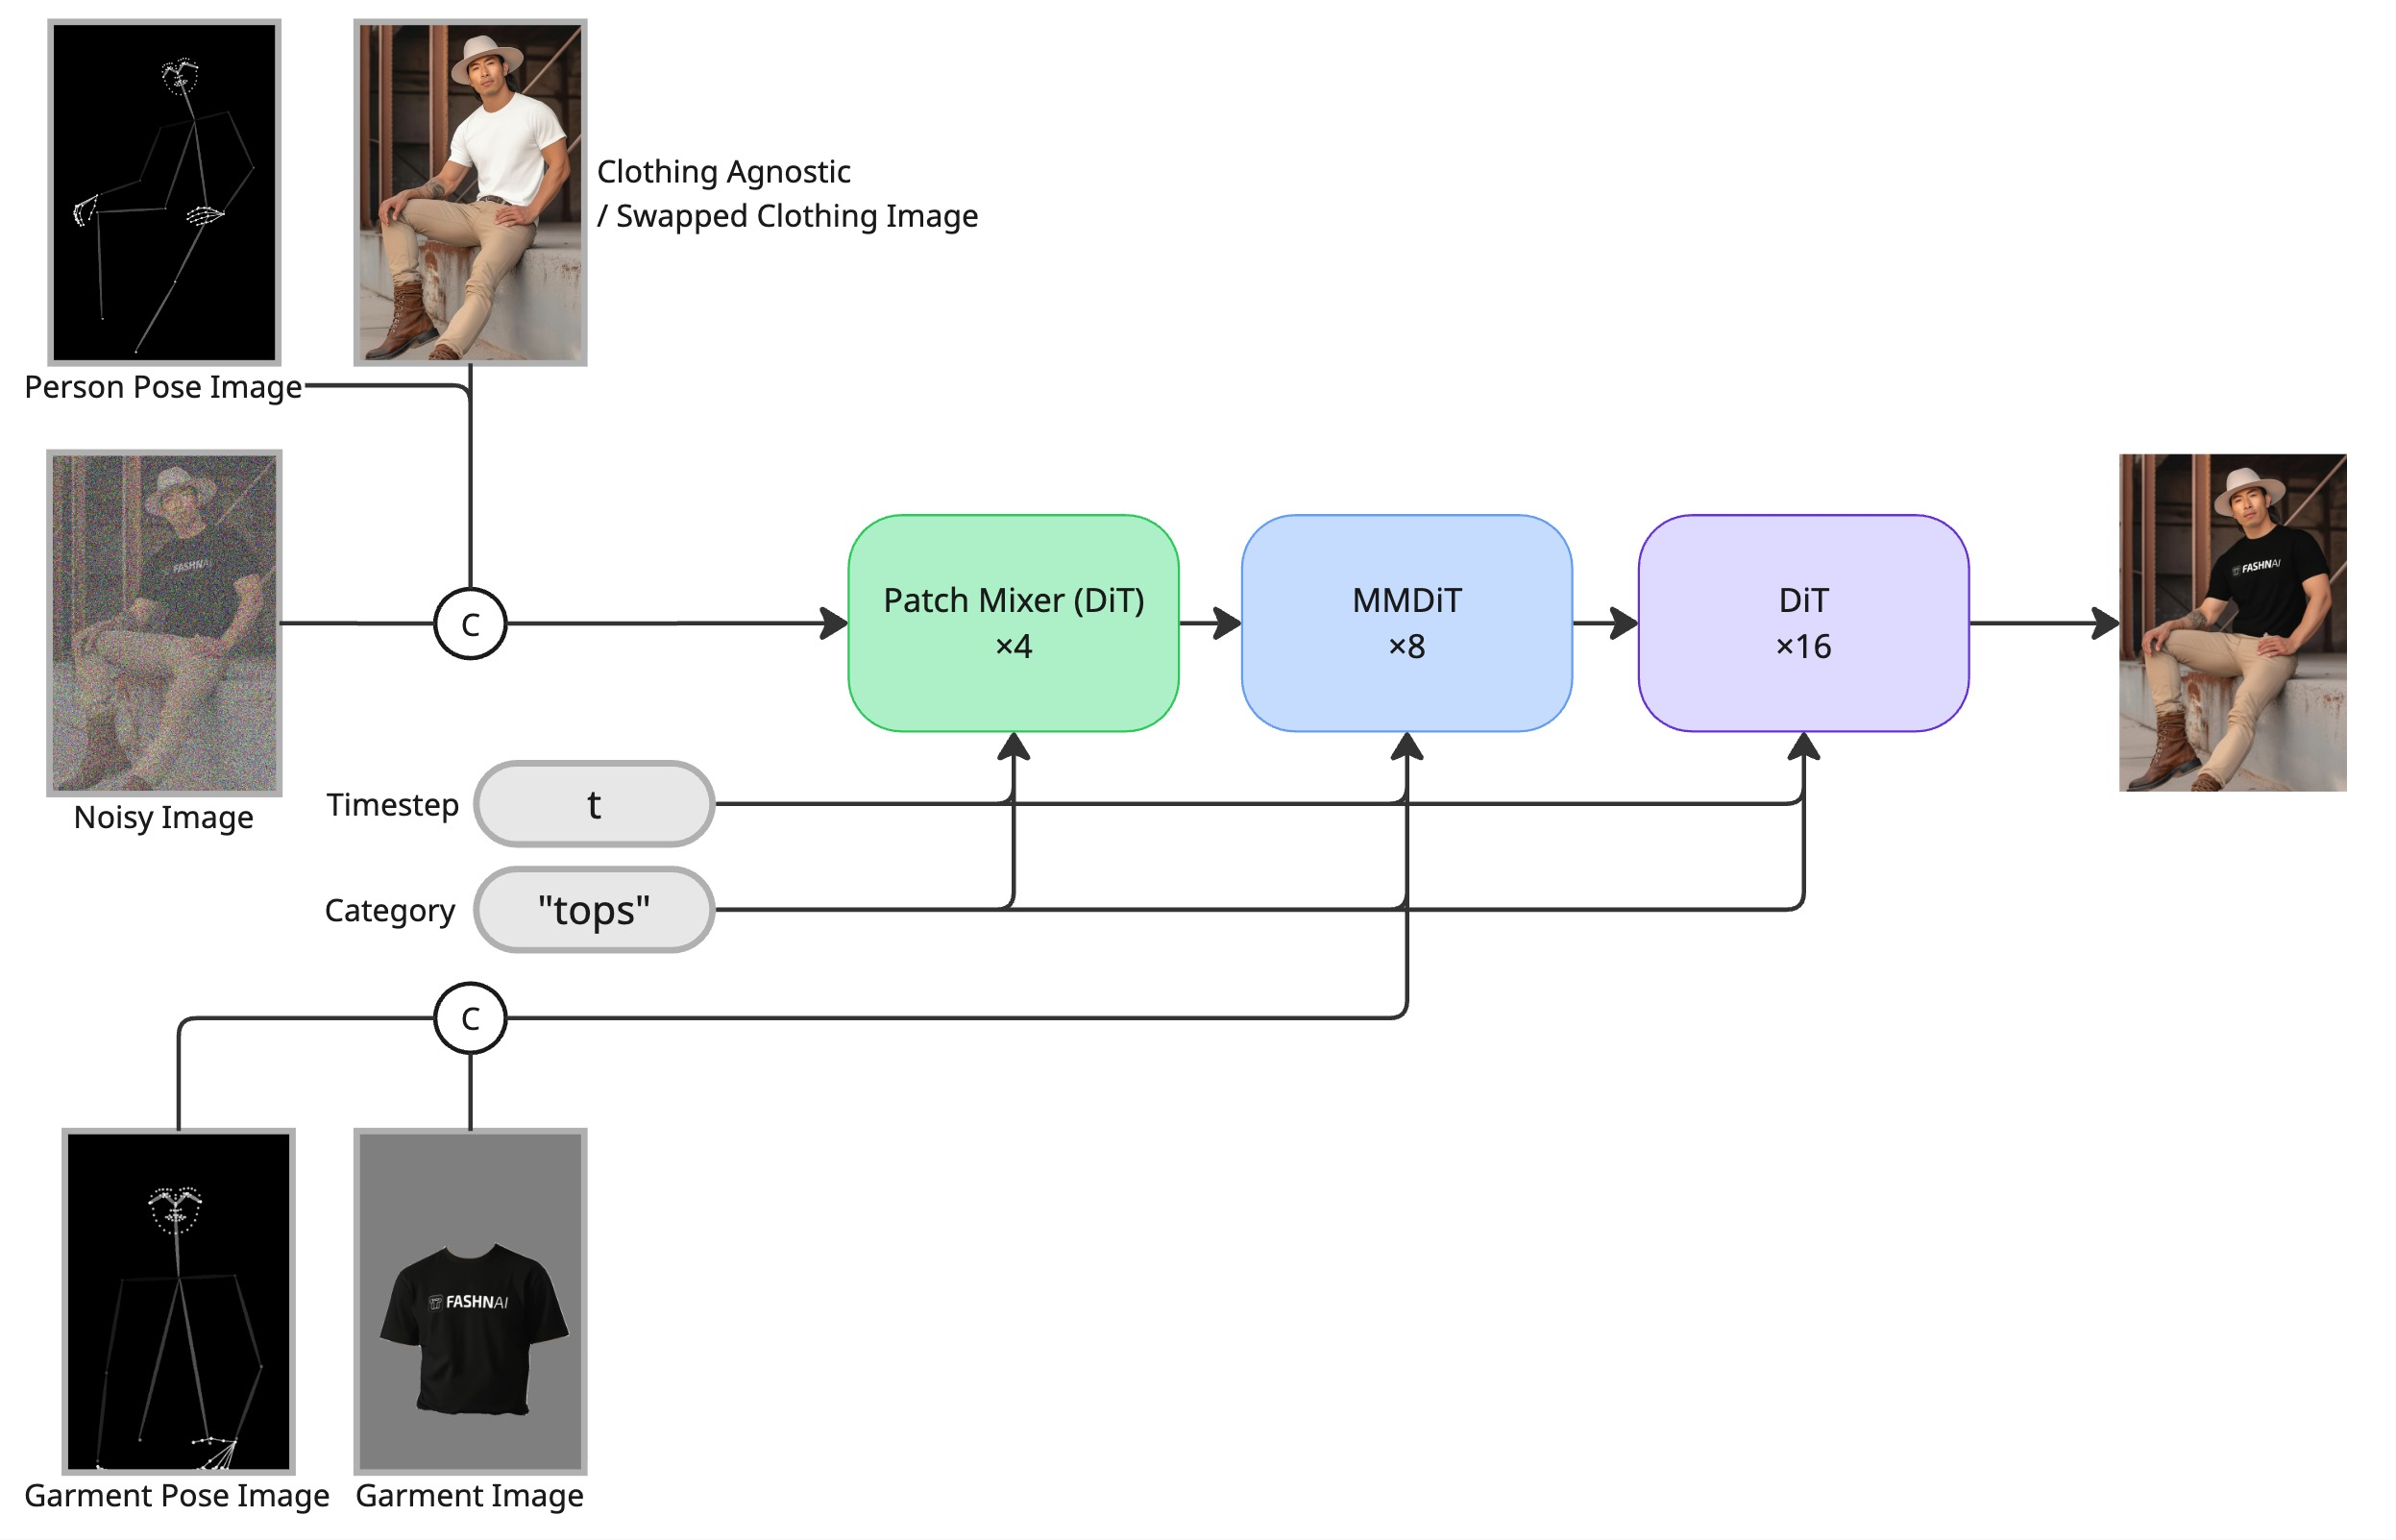
\includegraphics[width=\linewidth]{fashn-vton-diagram.jpg}
  \caption[FASHN VTON v1.5 model flow]{FASHN VTON v1.5 model flow. Pose, garment conditioning, timestep và category information đi qua Patch Mixer, MMDiT và DiT blocks trước khi tạo ảnh try-on. Source: FASHN VTON v1.5 research page.}
\end{figure}

FASHN router là abstraction boundary:

\begin{itemize}
  \item Đọc GPU assignment từ configuration.
  \item Tạo worker definition theo từng GPU được cấu hình.
  \item Pin mỗi worker vào một CUDA device.
  \item Dùng Unix socket để tránh mở public worker port.
  \item Thực hiện readiness check.
  \item Route request bằng least-inflight kết hợp round-robin.
  \item Expose Prometheus metrics với label \code{worker_id}, \code{gpu_id}, \code{gpu_uuid} và \code{status}.
  \item Ghi structured router và worker logs.
\end{itemize}

\section{VTON Job Lifecycle}

\begin{enumerate}
  \item User upload person image và garment image.
  \item API normalize và lưu image artifacts.
  \item User submit VTON job.
  \item API kiểm tra payload, auth, quota và workspace concurrency.
  \item VTON job queue lưu job snapshot.
  \item Runner gọi VTON inference implementation.
  \item Adapter gọi FASHN router endpoint.
  \item FASHN worker tạo output PNG và report metadata.
  \item API lưu request record và job result.
  \item UI poll job status và mở output artifact.
\end{enumerate}

\begin{center}
\begin{tabular}{ll}
\toprule
\textbf{Status} & \textbf{Ý nghĩa} \\
\midrule
accepted & API nhận job \\
queued & Job đang chờ trong queue \\
running & Job đang thực thi \\
completed & Job có output artifact \\
failed & Job lỗi và có error message \\
\bottomrule
\end{tabular}
\end{center}

\section{Multi-GPU Worker Configuration}

Trong multi-GPU deployment, router được cấu hình bằng danh sách GPU identifier có thể sử dụng. Mỗi worker gắn với một GPU và giao tiếp qua private endpoint. Product API chỉ gọi router, còn Prometheus/Grafana quan sát worker behavior qua label về worker identity, GPU identity, request status, latency và in-flight count.

\begin{center}
\begin{tabular}{lll}
\toprule
\textbf{Worker} & \textbf{CUDA pin} & \textbf{Private endpoint} \\
\midrule
\code{fashn-gpu0} & \code{CUDA_VISIBLE_DEVICES=0} & Unix socket \\
\code{fashn-gpu1} & \code{CUDA_VISIBLE_DEVICES=1} & Unix socket \\
\code{fashn-gpu2} & \code{CUDA_VISIBLE_DEVICES=2} & Unix socket \\
\bottomrule
\end{tabular}
\end{center}

API và Prometheus không cần biết private worker endpoint. Chúng giao tiếp qua router. Grafana vẫn hiển thị được per-worker activity vì router phát metrics có worker và GPU labels.

\section{LLM Serving}

LLM serving dùng OpenAI-compatible adapter. Adapter gọi chat-completions interface và ghi lại:

\begin{itemize}
  \item model name,
  \item provider/base URL sau khi sanitize,
  \item input và output token count,
  \item latency,
  \item tokens per second,
  \item estimated cost khi có cấu hình,
  \item guardrail flags,
  \item structured output validation khi request yêu cầu.
\end{itemize}

Thiết kế này cho phép thay đổi provider hoặc self-hosted endpoint mà không làm thay đổi product workflow.

% ---------------------------------------------------------------------------
\chapter{Governance, Security và Responsible AI}
% ---------------------------------------------------------------------------

\section{Authentication và Workspace Model}

TryOps dùng Keycloak làm OIDC identity provider. Browser đăng nhập bằng authorization code flow với PKCE. Gateway validate token và forward principal metadata tới backend. Khi user đăng nhập lần đầu, backend bootstrap workspace account trong Postgres.

\screenshotfig{screenshots/keycloak.png}{Keycloak session control và identity surface}

\section{Quota và Admission Control}

Quota được kiểm soát ở hai lớp:

\begin{itemize}
  \item Rust gateway thực hiện edge quota/rate admission.
  \item FastAPI backend thực hiện workload-level VTON workspace concurrency.
\end{itemize}

\begin{center}
\begin{tabular}{lr}
\toprule
\textbf{Plan} & \textbf{Active VTON jobs} \\
\midrule
free & 1 \\
team & 2 \\
enterprise & 4 \\
\bottomrule
\end{tabular}
\end{center}

Plan limit khác với GPU worker count. Một workspace có thể bị giới hạn một active job dù router có nhiều GPU worker.

\section{Guardrail}

Guardrail chạy tại gateway và API boundary:

\begin{itemize}
  \item Prompt injection detection.
  \item System prompt leakage prevention.
  \item PII và secret-like string masking.
  \item Output size và structured output validation.
  \item Metrics theo risk category.
\end{itemize}

Go guardrail service được gọi qua internal service URL đã cấu hình.

\section{Promotion Gate}

Model promotion yêu cầu:

\begin{itemize}
  \item model card,
  \item data card,
  \item evaluation report,
  \item SBOM,
  \item model artifact scan,
  \item provenance attestation,
  \item risk controls,
  \item owner approvals,
  \item policy verdict.
\end{itemize}

\begin{center}
\begin{tabular}{ll}
\toprule
\textbf{State} & \textbf{Ý nghĩa} \\
\midrule
candidate & Output từ pipeline, chưa được tin cậy để promote \\
challenger & Đã qua staging gate, có thể shadow/canary \\
champion & Model đang được promote \\
rejected & Bị policy chặn \\
archived & Giữ lại cho audit và rollback history \\
\bottomrule
\end{tabular}
\end{center}

\section{Supply Chain và Privacy}

Repository chứa tài liệu về model source, dependency inventory, dataset licensing và promotion decision. Production logs không nên lưu raw prompt, raw uploaded image hoặc provider secret. Logs nên tham chiếu artifact ID, request ID, trace ID và job ID để hỗ trợ debugging mà vẫn giữ privacy.

% ---------------------------------------------------------------------------
\chapter{Observability và Vận hành}
% ---------------------------------------------------------------------------

\section{Dashboard}

\begin{longtable}{p{5cm}p{9.8cm}}
\toprule
\textbf{Dashboard} & \textbf{Mục đích} \\
\midrule
TryOps Service Overview & Request rate, error ratio, latency, memory, queue depth, gateway errors \\
TryOps Model Quality & Quality score, VTON latency, LLM throughput, completed inference \\
TryOps Cost and Capacity & Cost, quota utilization, cache hit rate, energy/carbon \\
TryOps Guardrails & Blocked/redacted/reviewed findings theo risk category \\
TryOps Observability Drilldown & Logs, job lifecycle, FASHN service logs, OTel/Tempo/Loki health \\
\bottomrule
\end{longtable}

\section{Logs}

Các nhóm log quan trọng:

\begin{itemize}
  \item API request và job lifecycle events.
  \item FASHN router events.
  \item Per-worker VTON inference events.
  \item Model-serving process logs.
  \item Trace spans cho API và background jobs.
\end{itemize}

Grafana nên cho phép tìm log theo job ID, request ID, account ID, worker ID và GPU ID. Điều này cần thiết cho các tình huống UI đang chờ nhưng backend đã hoàn thành hoặc đã ghi lỗi job.

\section{Metrics}

Các nhóm metric quan trọng:

\begin{itemize}
  \item HTTP request count và duration theo service/status.
  \item VTON job lifecycle counter và active queue depth.
  \item FASHN router worker request và in-flight count.
  \item Per-worker latency và failure count.
  \item LLM token throughput, latency và error rate.
  \item Guardrail block/redaction counters.
  \item Quota admission và remaining capacity.
  \item Hardware usage từ host exporter và GPU exporter.
\end{itemize}

\section{Developer-Local Ports}

Trong developer-local stack, nhiều port được expose để debug nhanh. Với shared datacenter, thiết kế nên thu hẹp public surface: gateway, Keycloak và Grafana dành cho operator; database, object store, metrics backend, guardrail và model endpoint nằm trong private network.

\clearpage
\begin{figure}[p]
\centering
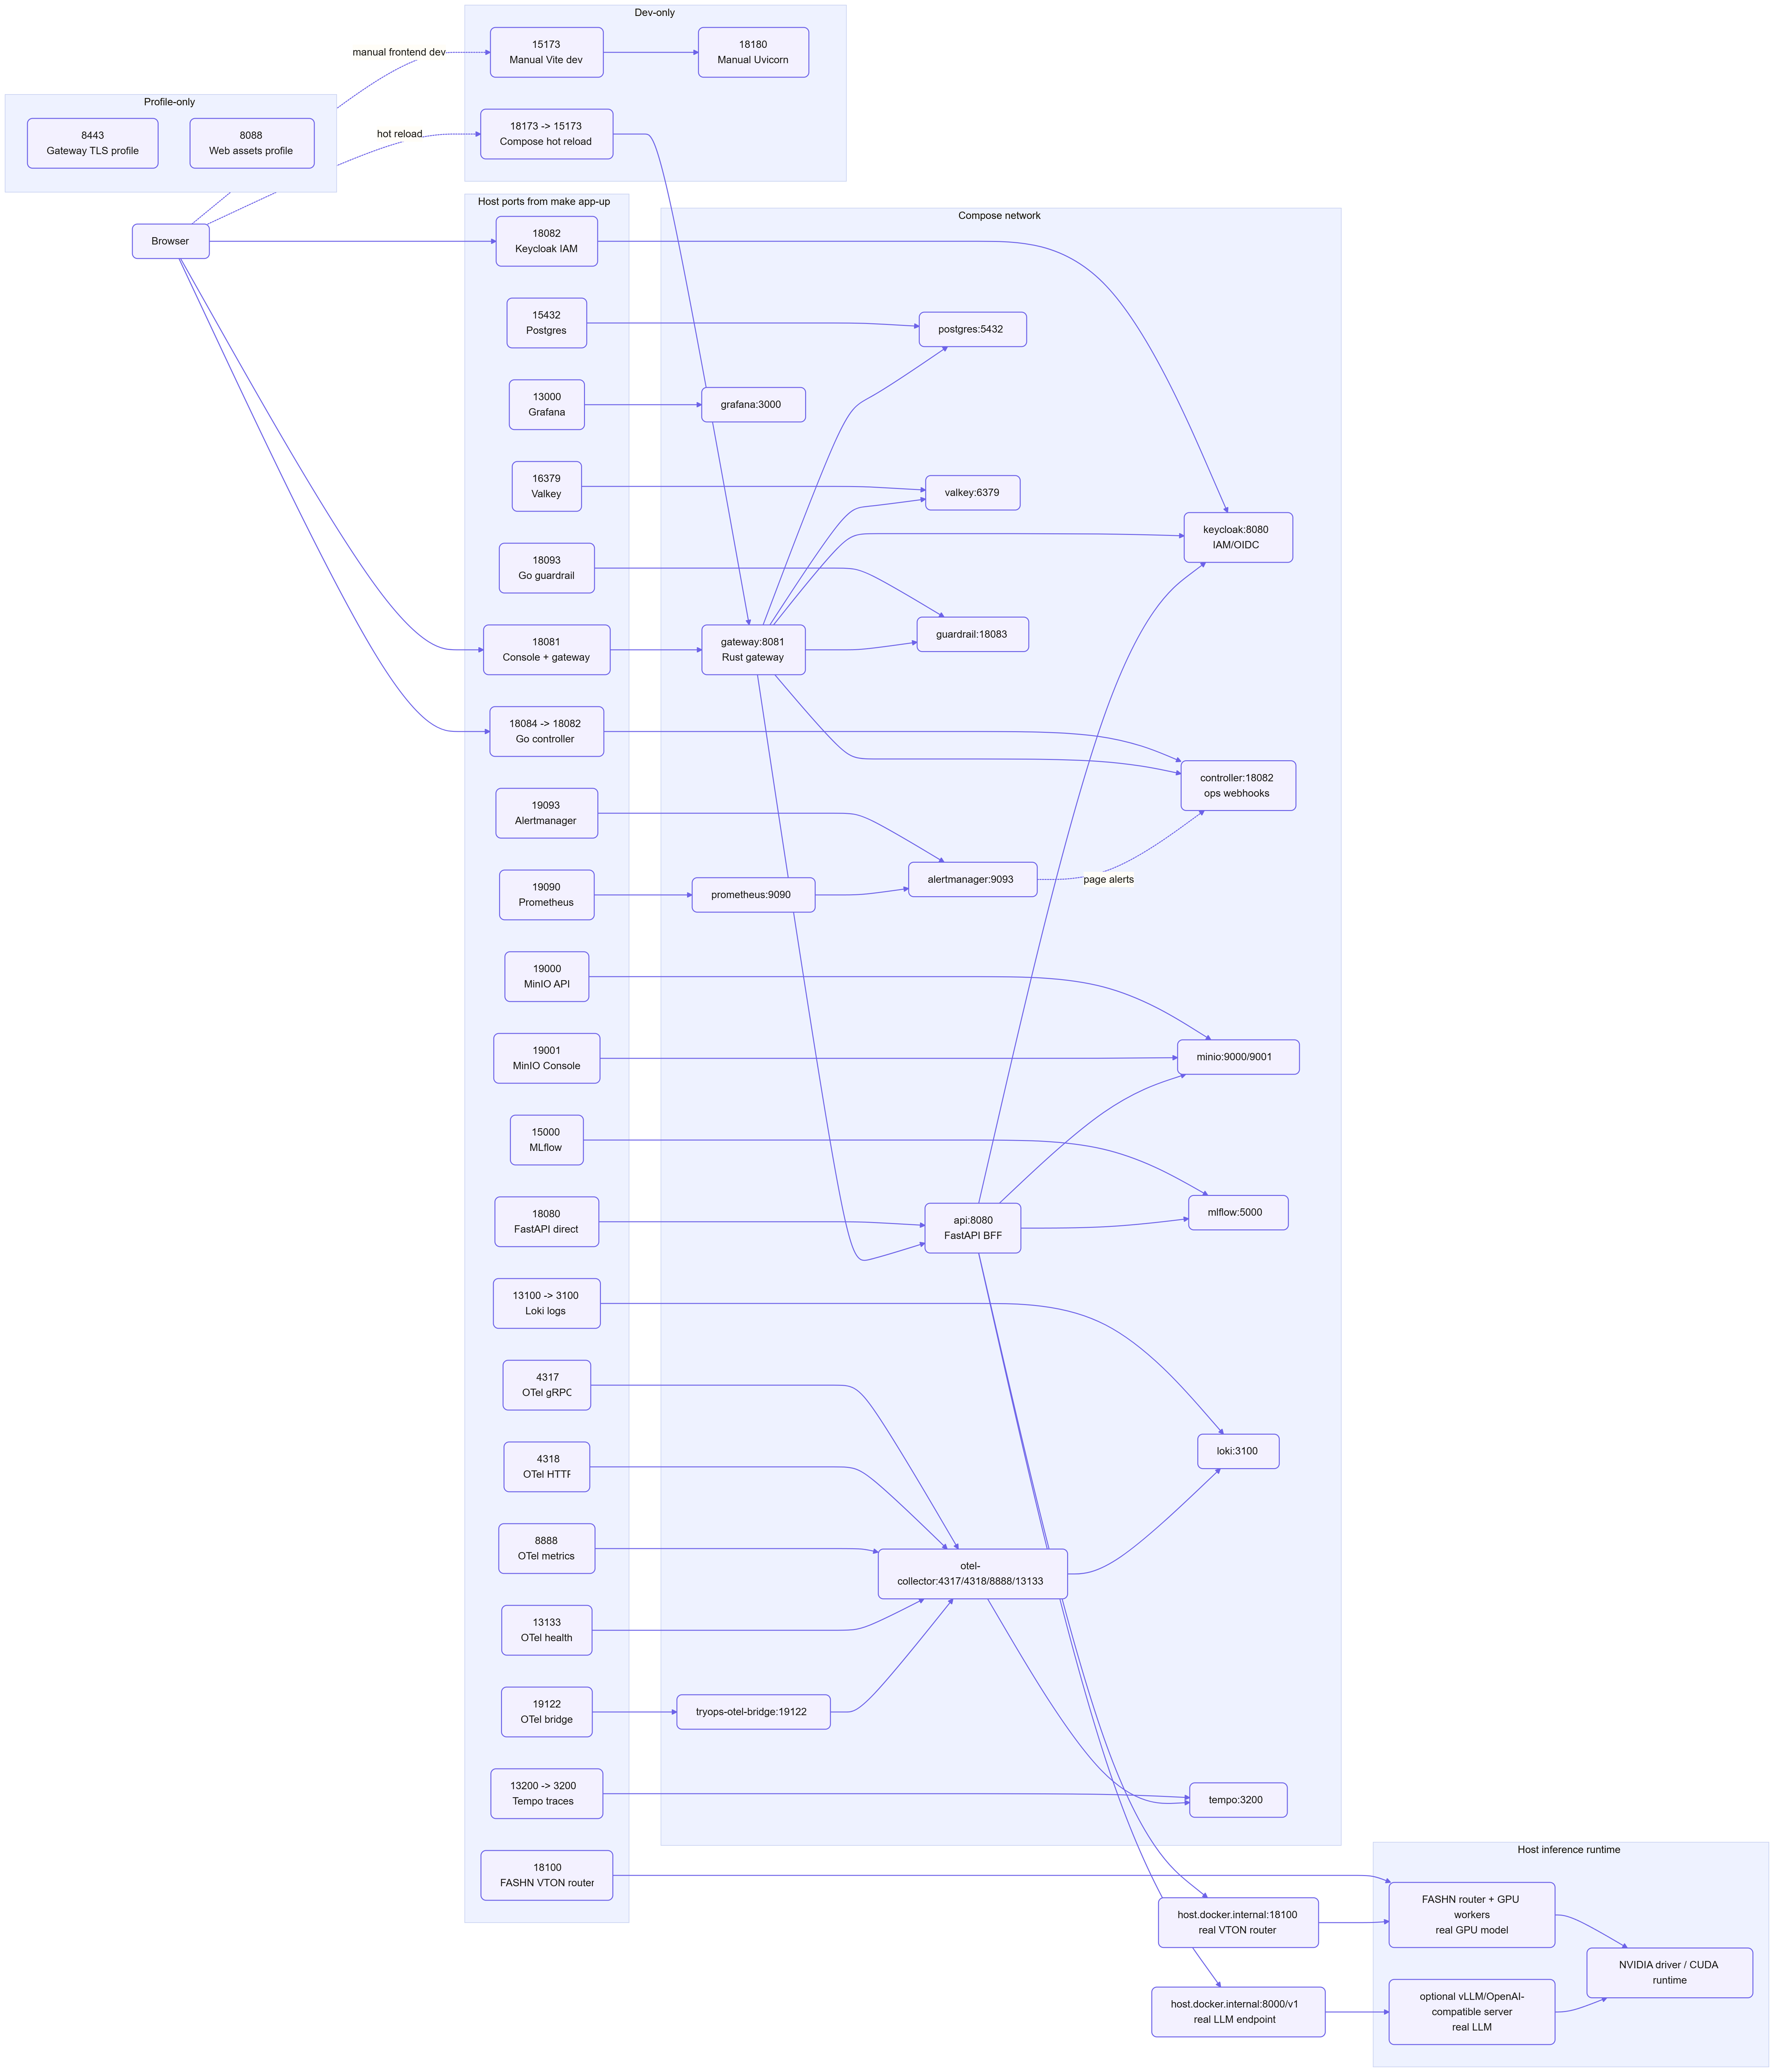
\includegraphics[width=\linewidth,height=0.88\textheight,keepaspectratio]{port-service-diagram.png}
\caption{Developer-local service topology và quan hệ giữa host port, Compose network và host inference runtime.}
\label{fig:port-service-diagram-vi}
\end{figure}
\clearpage

\begingroup
\scriptsize
\setlength{\tabcolsep}{2.5pt}
\renewcommand{\arraystretch}{1.16}
\begin{longtable}{>{\raggedright\arraybackslash}p{3.35cm}>{\raggedright\arraybackslash}p{1.25cm}>{\raggedright\arraybackslash}p{3.95cm}>{\raggedright\arraybackslash}p{6.35cm}}
\caption{Developer-local \code{make app-up} ports và override variables.}
\label{tab:developer-local-ports-vi}\\
\toprule
\textbf{Service} & \textbf{Port} & \textbf{Override variable} & \textbf{Notes} \\
\midrule
\endfirsthead
\toprule
\textbf{Service} & \textbf{Port} & \textbf{Override variable} & \textbf{Notes} \\
\midrule
\endhead
TryOps Console + Rust gateway & \code{18081} & \code{TRYOPS_GATEWAY_PORT} & Main app URL. Nên dùng entry point này trước. \\
FastAPI backend direct & \code{18080} & \code{TRYOPS_API_PORT} & Direct API/docs access. Gateway thường proxy service này. \\
Keycloak IAM & \code{18082} & \code{TRYOPS_KEYCLOAK_PORT} & OIDC/IAM service. Container port là \code{8080}. \\
Go controller & \code{18084} & \code{TRYOPS_CONTROLLER_PORT} & Webhook/control-plane service. Container port là \code{18082}; Alertmanager gọi \code{controller:18082/alerts/webhook} trong Compose. \\
FASHN VTON router & \code{18100} & \code{FASHN_VTON_ROUTER_PORT} & Host-side VTON router được \code{make app-up} khởi động. API gọi qua \code{host.docker.internal:18100}. \\
FASHN VTON single-worker debug & \code{18101} & \code{FASHN_VTON_PORT} & Direct service dùng cho isolated debugging với \code{make fashn-vton-service-bg}. \code{make app-up} không dùng path này. \\
Optional local vLLM/OpenAI-compatible LLM & \code{8000} & \code{VLLM_PORT}\newline\code{VLLM_BASE_URL}\newline\code{TRYOPS_LLM_BASE_URL} & Host-side LLM endpoint khi self-host vLLM. Nếu \code{TRYOPS_LLM_BASE_URL} trỏ tới external provider, không cần local LLM port. \\
Postgres & \code{15432} & \code{TRYOPS_POSTGRES_PORT} & Database cho full Compose stack. \\
Valkey & \code{16379} & \code{TRYOPS_VALKEY_PORT} & Hot quota và rate-counter store. \\
MinIO API & \code{19000} & \code{TRYOPS_MINIO_PORT} & Object và artifact storage API. \\
MinIO Console & \code{19001} & \code{TRYOPS_MINIO_CONSOLE_PORT} & Browser UI cho MinIO. \\
MLflow & \code{15000} & \code{TRYOPS_MLFLOW_PORT} & Experiment và model tracking. \\
Prometheus & \code{19090} & \code{TRYOPS_PROMETHEUS_PORT} & Metrics database. \\
Alertmanager & \code{19093} & \code{TRYOPS_ALERTMANAGER_PORT} & Alert routing. \\
Grafana & \code{13000} & \code{TRYOPS_GRAFANA_PORT} & Dashboards. Local volume mới thường dùng \code{admin} / \code{admin}. \\
Loki & \code{13100} & \code{TRYOPS_LOKI_PORT} & Log store cho Grafana khi observability được bật. Container port là \code{3100}. \\
Tempo & \code{13200} & \code{TRYOPS_TEMPO_PORT} & Trace store cho Grafana khi observability được bật. Container port là \code{3200}. \\
Go guardrail sidecar & \code{18093} & \code{TRYOPS_GUARDRAIL_PORT} & LLM guardrail service. Thường được gọi bởi gateway/API. Container port là \code{18083}. \\
OpenTelemetry gRPC & \code{4317} & \code{TRYOPS_OTEL_GRPC_PORT} & OTLP gRPC receiver. \\
OpenTelemetry HTTP & \code{4318} & \code{TRYOPS_OTEL_HTTP_PORT} & OTLP HTTP receiver. \\
OpenTelemetry metrics & \code{8888} & \code{TRYOPS_OTEL_METRICS_PORT} & Collector metrics endpoint. \\
OpenTelemetry health & \code{13133} & \code{TRYOPS_OTEL_HEALTH_PORT} & Collector health endpoint. \\
OTel bridge metrics & \code{19122} & \code{TRYOPS_OTEL_BRIDGE_PORT} & Metrics endpoint path là \code{/metrics}. Bridge local TryOps JSONL logs/traces vào OTLP để Grafana, Loki và Tempo đọc được. \\
\bottomrule
\end{longtable}
\endgroup
\clearpage

\section{Deployment Preconditions}

Deployment hướng tới production cần có model endpoints được cấu hình, provider credentials được bảo vệ, development shortcut bị tắt và GPU readiness check rõ ràng cho VTON inference. Operational checks nên xác minh service health, authentication, quota admission, object storage, observability và model-serving readiness trước khi cho user submit inference job tốn tài nguyên.

% ---------------------------------------------------------------------------
\chapter{Thực nghiệm và đánh giá}
% ---------------------------------------------------------------------------

\section{VTON Benchmark Results}

\begin{center}
\metriccard[TryOpsTeal]{0.29\linewidth}{Best quality score}{0.888121 SSIM}
\hfill
\metriccard[TryOpsTeal]{0.29\linewidth}{Best image fidelity}{18.915 PSNR}
\hfill
\metriccard[TryOpsTeal]{0.29\linewidth}{Lowest VTON memory}{4.825 GB VRAM}

\vspace{0.45em}

\metriccard[TryOpsBlue]{0.43\linewidth}{Fastest average latency}{17,842.30 ms}
\hfill
\metriccard[TryOpsBlue]{0.43\linewidth}{Highest VTON throughput}{0.054261 req/s}
\end{center}

\begin{table}[H]
\centering
\caption{Kết quả benchmark VTON dùng cho model selection.}
\label{tab:vton-benchmark-vi}
\renewcommand{\arraystretch}{1.22}
\small
\resizebox{\linewidth}{!}{%
\begin{tabular}{lrrrrrrrr}
\toprule
\textbf{Candidate} & \textbf{SSIM} & \textbf{PSNR} & \textbf{Avg ms} & \textbf{P95 ms} & \textbf{req/s} & \textbf{Model ms} & \textbf{GPU \%} & \textbf{VRAM GB} \\
\midrule
\textbf{FASHN VTON v1.5} & \metric[TryOpsTeal]{0.888121} & \metric[TryOpsTeal]{18.915} & 21,337.50 & 23,244.00 & 0.045439 & 19,969.60 & \metric[TryOpsGold]{100.00} & \metric[TryOpsTeal]{4.825} \\
CatVTON & 0.861734 & 18.284 & \metric[TryOpsBlue]{17,842.30} & \metric[TryOpsBlue]{19,604.00} & \metric[TryOpsBlue]{0.054261} & \metric[TryOpsBlue]{16,512.80} & 96.50 & 6.742 \\
IDM-VTON & 0.879462 & 18.671 & 42,586.70 & 47,918.00 & 0.022751 & 40,318.40 & 99.20 & 13.684 \\
OOTDiffusion & 0.852918 & 17.936 & 35,214.90 & 39,876.00 & 0.027502 & 33,087.60 & 98.40 & 10.927 \\
\bottomrule
\end{tabular}%
}

\vspace{0.45em}
\begin{minipage}{0.94\linewidth}
\footnotesize
\textbf{Cách đọc kết quả.} FASHN VTON v1.5 là candidate mạnh nhất theo hướng ưu tiên quality vì có SSIM, PSNR và VRAM tốt nhất trong bảng. CatVTON là candidate mạnh nhất theo hướng latency/throughput, nhưng quality metrics thấp hơn.
\end{minipage}
\end{table}

\begin{figure}[H]
\centering
\small
\begin{tabularx}{\linewidth}{>{\raggedright\arraybackslash}X>{\raggedright\arraybackslash}X>{\raggedright\arraybackslash}X}
\toprule
\textbf{Best quality} & \textbf{Best latency} & \textbf{Heavier candidates} \\
\midrule
FASHN VTON v1.5 dẫn đầu SSIM và PSNR trong recorded run, đồng thời dùng ít GPU memory nhất. &
CatVTON có average latency, P95 latency, model latency thấp nhất và throughput cao nhất. &
IDM-VTON và OOTDiffusion tốn latency, VRAM và host RAM hơn trong benchmark này. \\
\bottomrule
\end{tabularx}

\vspace{0.6em}
\scriptsize
\resizebox{0.92\linewidth}{!}{%
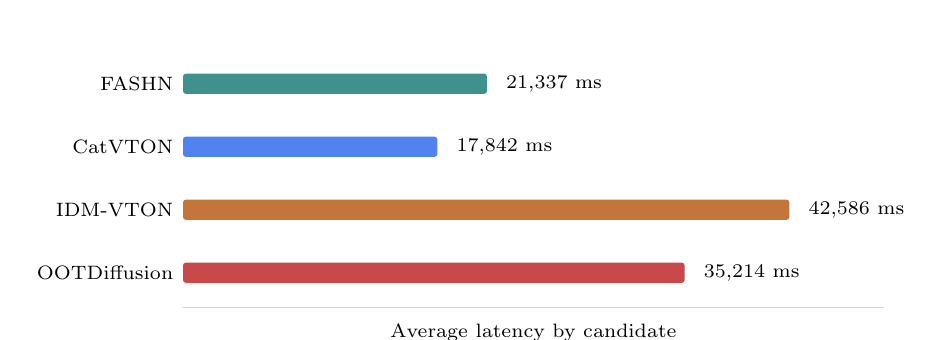
\begin{tikzpicture}[
  x=1cm,
  y=0.80cm,
  every node/.style={font=\scriptsize},
  bar/.style={draw=none, rounded corners=1pt}
]
\node[anchor=east] at (0,3) {FASHN};
\fill[bar, TryOpsTeal!80] (0,2.84) rectangle (3.86,3.16);
\node[anchor=west] at (3.98,3) {21,337 ms};

\node[anchor=east] at (0,2) {CatVTON};
\fill[bar, TryOpsBlue!80] (0,1.84) rectangle (3.23,2.16);
\node[anchor=west] at (3.35,2) {17,842 ms};

\node[anchor=east] at (0,1) {IDM-VTON};
\fill[bar, TryOpsGold!80] (0,0.84) rectangle (7.70,1.16);
\node[anchor=west] at (7.82,1) {42,586 ms};

\node[anchor=east] at (0,0) {OOTDiffusion};
\fill[bar, TryOpsRed!80] (0,-0.16) rectangle (6.37,0.16);
\node[anchor=west] at (6.49,0) {35,214 ms};

\draw[TryOpsLine] (0,-0.55) -- (8.90,-0.55);
\node[anchor=north] at (4.45,-0.66) {Average latency by candidate};
\end{tikzpicture}%
}
\caption{Diễn giải benchmark VTON và so sánh average latency.}
\end{figure}

\section{LLM Optimization Results}

LLM optimization summary ghi lại Pareto frontier giữa memory và decode speed:

\begin{table}[H]
\centering
\caption{Các đo đạc LLM optimization đáng chú ý.}
\small
\begin{tabularx}{\linewidth}{>{\bfseries}p{2.2cm}p{3.1cm}p{3.1cm}X}
\toprule
\textbf{Mode} & \textbf{VRAM} & \textbf{Decode speed} & \textbf{Nhận xét} \\
\midrule
fp16 & \metric[TryOpsBlue]{1.010 GB} & \metric[TryOpsTeal]{27.4 tokens/s} & Decode speed cao nhất trong recorded run. \\
8-bit & \metric[TryOpsGold]{0.647 GB} & \metric[TryOpsRed]{5.9 tokens/s} & Memory thấp hơn fp16, nhưng chậm hơn trong lần đo này. \\
4-bit & \metric[TryOpsTeal]{0.478 GB} & \metric[TryOpsBlue]{13.9 tokens/s} & Low-memory option tốt hơn 8-bit trong bảng so sánh này. \\
\bottomrule
\end{tabularx}
\end{table}

Bài học vận hành là lower precision không tự động đồng nghĩa với tổng chi phí thấp hơn. Nếu quantized model decode chậm hơn nhiều trong khi board power tương tự, joules per token và rental cost per million tokens có thể tăng.

\section{Native Boundary Evaluation}

Go load driver ghi nhận Rust \code{/health} đạt \metric[TryOpsTeal]{24,840.8 requests/s}, trong khi FastAPI đạt \metric[TryOpsGold]{1,539.4 requests/s} trên cùng máy, chênh lệch khoảng \metric[TryOpsBlue]{16.1x}. Điều này không có nghĩa là loại bỏ Python. Python vẫn phù hợp cho ML workflow, còn Rust/Go/C++ hỗ trợ edge, control plane và native tooling.

\section{Balancer Testing}

Kiểm thử router multi-GPU nên gửi nhiều request đồng thời vào router và xác minh completed-request counters tăng trên nhiều worker/GPU label. Nếu chỉ một GPU nhận việc, các điểm cần kiểm tra trước gồm workspace job concurrency, API job worker count, router worker readiness, GPU assignment và số lượng request đồng thời có đủ để vượt một worker in-flight hay không.

% ---------------------------------------------------------------------------
\chapter{Giới hạn và hướng phát triển}
% ---------------------------------------------------------------------------

\section{Giới hạn hiện tại}

\begin{itemize}
  \item Chưa thể hot-reload để tự động deploy model mới dựa trên MLFlow.
  \item Live vLLM benchmark phụ thuộc host environment và serving runtime đang được cài đặt.
  \item KServe/Kubeflow cluster deployment là target profile, chưa phải local stack đang đóng gói.
  \item Tối ưu quá mạnh VTON model có thể tạo output bị mờ, mất texture và không đạt yêu cầu thị giác; VTON deployment cần image-quality regression tests, không chỉ kiểm tra API success.
  \item Một số operator workflow trong UI cần thêm click-through detail và export feature.
  \item Shared-datacenter port reduction cần hoàn thiện bằng cách đưa internal services vào ingress/private network.
  \item GPU utilization dashboard cần host GPU exporter và per-worker router metrics được scrape ổn định.
\end{itemize}

Một giới hạn cụ thể quan sát được khi tối ưu VTON là runtime setting quá mạnh có thể giữ được API success nhưng làm giảm chất lượng ảnh. Output có thể mờ ở vùng cơ thể và trang phục, texture không rõ, đường biên trang phục yếu. Vì vậy VTON promotion không thể chỉ dựa vào HTTP success, latency và GPU memory; cần thêm quality gate cho ảnh sinh ra.

\begin{figure}[H]
  \centering
  
\includegraphics[width=0.42\linewidth]{blur_vton.png}
  \caption[VTON optimization limitation]{Giới hạn khi tối ưu VTON: output bị mờ ở vùng trang phục và cơ thể, cho thấy optimized variant cần image-quality gate trước khi promotion.}
\end{figure}

\section{Hướng phát triển}

\begin{enumerate}
  \item Có thể hot-reload để tự động deploy model mới dựa trên MLFlow gateway, và có thuật toán promotion gate reload để hạn chế downtime.
  \item Harden shared-host deployment với public port surface tối thiểu.
  \item Tích hợp host GPU exporter và Grafana GPU worker dashboard.
  \item Tích hợp production secret manager.
  \item Mở rộng VTON evaluation bằng human preference labels và fairness slices.
  \item Bổ sung compatibility tests cho nhiều LLM provider/model.
  \item Đóng gói KServe/Kubeflow profile cho cluster-grade deployment.
  \item Cải thiện incident response runbook và dashboard drilldown.
\end{enumerate}

% ---------------------------------------------------------------------------
\chapter{Kết luận}
% ---------------------------------------------------------------------------

TryOps trình bày một nền tảng MLOps xem model như production asset có quản trị, thay vì chỉ là output của notebook. Đồ án tích hợp product console, model-serving boundary, account/quota control, artifact storage, model governance, observability, native control-plane components và readiness checks.

Kết quả quan trọng nhất là kiến trúc: VTON và LLM có thể dùng chung một operational spine nhưng vẫn giữ nhu cầu riêng của từng workload. VTON cần GPU-aware job control, image artifact lineage và image-quality assessment. LLM serving cần token accounting, endpoint health, guardrail và latency/cost measurement. TryOps dùng cùng gateway, API, observability, storage và governance foundation cho cả hai.

Hệ thống vẫn cần được harden thêm trước khi vận hành như một multi-tenant data-center platform. Tuy vậy, thiết kế hiện tại đã thể hiện các phần cốt lõi của MLOps: model change phải đi qua promotion gate, operator có đủ logs/metrics/traces để debug, artifact và lineage được lưu lại, còn các utility dùng cho testing/evaluation được tách khỏi product path.

\phantomsection
\addcontentsline{toc}{chapter}{Tài liệu tham khảo}
\begin{thebibliography}{99}

\bibitem{opentelemetry}
OpenTelemetry, ``OpenTelemetry Documentation,'' [Online]. Available:
\url{https://opentelemetry.io/docs/}. Accessed: July 4, 2026.

\bibitem{prometheus}
Prometheus Authors, ``Prometheus Documentation,'' [Online]. Available:
\url{https://prometheus.io/docs/}. Accessed: July 4, 2026.

\bibitem{grafana}
Grafana Labs, ``Grafana Documentation,'' [Online]. Available:
\url{https://grafana.com/docs/grafana/latest/}. Accessed: July 4, 2026.

\bibitem{loki}
Grafana Labs, ``Grafana Loki Documentation,'' [Online]. Available:
\url{https://grafana.com/docs/loki/latest/}. Accessed: July 4, 2026.

\bibitem{tempo}
Grafana Labs, ``Grafana Tempo Documentation,'' [Online]. Available:
\url{https://grafana.com/docs/tempo/latest/}. Accessed: July 4, 2026.

\bibitem{fastapi}
FastAPI, ``FastAPI Documentation,'' [Online]. Available:
\url{https://fastapi.tiangolo.com/}. Accessed: July 4, 2026.

\bibitem{mlflow}
MLflow, ``MLflow Documentation,'' [Online]. Available:
\url{https://mlflow.org/docs/latest/}. Accessed: July 4, 2026.

\bibitem{minio}
MinIO, ``MinIO Object Storage Documentation,'' [Online]. Available:
\url{https://min.io/docs/minio/linux/}. Accessed: July 4, 2026.

\bibitem{keycloak}
Keycloak, ``Keycloak Documentation,'' [Online]. Available:
\url{https://www.keycloak.org/documentation}. Accessed: July 4, 2026.

\bibitem{fashn-vton}
FASHN, ``FASHN VTON 1.5 Research,'' [Online]. Available:
\url{https://fashn.ai/research/vton-1-5}. Accessed: July 4, 2026.

\bibitem{vllm}
vLLM Project, ``vLLM Documentation,'' [Online]. Available:
\url{https://docs.vllm.ai/}. Accessed: July 4, 2026.

\bibitem{openai-api}
OpenAI, ``OpenAI API Documentation,'' [Online]. Available:
\url{https://platform.openai.com/docs/}. Accessed: July 4, 2026.

\bibitem{nist-ai-rmf}
National Institute of Standards and Technology, ``Artificial Intelligence Risk
Management Framework,'' [Online]. Available:
\url{https://www.nist.gov/itl/ai-risk-management-framework}. Accessed:
July 4, 2026.

\bibitem{owasp-llm}
OWASP Foundation, ``OWASP Top 10 for Large Language Model Applications,''
[Online]. Available:
\url{https://owasp.org/www-project-top-10-for-large-language-model-applications/}.
Accessed: July 4, 2026.

\bibitem{slsa}
OpenSSF, ``Supply-chain Levels for Software Artifacts,'' [Online]. Available:
\url{https://slsa.dev/}. Accessed: July 4, 2026.

\end{thebibliography}

\end{document}
